\documentclass[letterpaper,conference,10pt]{IEEEconf}
\IEEEoverridecommandlockouts
\overrideIEEEmargins                                      % Needed to meet printer requirements.
% The preceding line is only needed to identify funding in the first footnote. If that is unneeded, please comment it out.
\usepackage{cite}
\renewcommand{\citeleft}{\textcolor{blue}{[}}
\renewcommand{\citeright}{\textcolor{blue}{]}}


% \usepackage{biblatex}
% \addbibresource{references.bib}
\usepackage{amsmath,amssymb,amsfonts}
\usepackage{algorithmic}
\usepackage{graphicx}
\usepackage{caption, subcaption}
% \usepackage{textcomp}
\usepackage[dvipsnames]{xcolor}
\usepackage{mathtools}
\usepackage{tabularx}
% \usepackage{subfig}
\usepackage{statmath}
\usepackage{url}
\usepackage{svg}
\usepackage{tikz}
\usepackage{makecell}
\usetikzlibrary{shapes,arrows,tikzmark,calc,fit}

\usetikzlibrary{arrows.meta,fit}

% Colors
\definecolor{OliveGreen}{RGB}{0,200,25}
\newcommand{\red}[1]{\textcolor{red}{#1}}
\newcommand{\green}[1]{\textcolor{green}{#1}}
\newcommand{\darkgreen}[1]{\textcolor{OliveGreen}{#1}}
\newcommand{\blue}[1]{\textcolor{blue}{#1}}
\newcommand{\orange}[1]{\textcolor{orange}{#1}}

\definecolor{myred}{RGB}{255,108,107}
\definecolor{lightred}{RGB}{255,188,187}
\definecolor{myblue}{RGB}{81,127,255}
\definecolor{lightblue}{RGB}{151,197,255}
\definecolor{mygreen}{RGB}{40,136,83}
\definecolor{lightgreen}{RGB}{80,176,123}
\definecolor{green}{RGB}{51,224,200}
\definecolor{lejla}{RGB}{162,97,255}
\definecolor{orange}{RGB}{210,125,69}

\let\argmax\relax
\let\argmin\relax
\DeclareMathOperator*{\argmax}{arg\!max}
\DeclareMathOperator*{\argmin}{arg\!min}
\DeclareMathOperator{\sign}{sign}

\tikzset{block/.style={draw, fill=blue!10, rectangle, thick,
minimum height=3em, minimum width=2em},
sum/.style={draw, fill=white, circle, thick, node distance=1cm},
input/.style={coordinate},
output/.style={coordinate},
pinstyle/.style={pin edge={latex[],thick,black}},
arrow/.style={draw,thick,-{latex[]}},
line/.style={draw,thick,-},
triangle/.style={draw,fill=red!20,regular polygon,regular polygon sides=3}}

\def\eqref#1{\textcolor{blue}{(\ref{#1})}}
% \ifCLASSOPTIONcompsoc
%     \usepackage[caption=false, font=normalsize, labelfont=sf, textfont=sf]{subfig}
% \else
% \usepackage[caption=false, font=footnotesize]{subfig}
% \fi

% \usepackage{lipsum}


\def\BibTeX{{\rm B\kern-.05em{\sc i\kern-.025em b}\kern-.08em
    T\kern-.1667em\lower.7ex\hbox{E}\kern-.125emX}}

% Choose between colored or gray figures
\usepackage{graphicx}
% \graphicspath{{figures/}}
% \graphicspath{{figures_gray/}}

\makeatletter
\let\NAT@parse\undefined
\makeatother

\usepackage{hyperref}
\usepackage{cleveref}
\hypersetup{
    colorlinks,
    linkcolor=blue,
    urlcolor=blue,
    citecolor=blue,
    pdftitle={Safe Navigation with Episode-based Reinforcement Learning and Model Predictive Control},
}
\def\equationautorefname~#1\null{Equation (#1)\null}

\usepackage{booktabs}
\usepackage[linesnumbered]{algorithm2e}
\SetKwComment{Comment}{/* }{ */}
\RestyleAlgo{ruled}

\renewcommand\AlCapFnt{\normalfont}
\SetAlgorithmName{Algorithm}{}{}

\usepackage{multirow}


\newcommand{\BIN}{\begin{bmatrix}}
\newcommand{\BOUT}{\end{bmatrix}}
\newcommand{\eq}[1]{eq.~(\ref{eq:#1})}
\newcommand{\rk}[1]{\mbox{rank}(#1)}

\DeclareMathOperator*{\minimize}{\min.}
\newcommand{\st}{\mbox{s.t.}}
\newcommand{\half}{\frac{1}{2}}
\newcommand{\act}{\mathcal{A}}

\newcommand{\SO}[1]{\mbox{SO}(#1)}
\newcommand{\SE}[1]{\mbox{SE}(#1)}

\usepackage{siunitx}
\sisetup{detect-all}

\usepackage{blindtext}
\usepackage{tablefootnote}
\usepackage{stackengine}
\usepackage[shortcuts,acronym]{glossaries}
% ---------------------------------------------------------------------------------
% ---------------------------------------------------------------------------------

\begin{document}

\title{\LARGE \bf Safe Navigation with Episode-based Reinforcement Learning\\ and Model Predictive Control}



% \author{Dhimiter Pikuli$^{1,2*}$, Gerhard Neumann$^2$, Thierry Fraichard$^1$  and Pierre-Brice Wieber$^1$% <-this % stops a space
\author{John Doe%
% \thanks{$^1$Inria, Montbonnot-Saint-Martin, France.}%
% \thanks{$^2$Université Grenoble Alpes, Grenoble, France}%
% \thanks{$^3$Karlsruhe Institue of Technology, Karlsruhe, Germany}%
% \thanks{$^*$Corresponding author. E-mail: \href{mailto:dhimiter.pikuli@inria.fr}{{dhimiter.pikuli@inria.fr}}.}% <-this % stops a space }%
}

\newacronym{ai}{AI}{Artificial Intelligence}
\newacronym{ann}{ANN}{Artificial Neural Networks}
\newacronym{ml}{ML}{Machine Learning}
\newacronym{dl}{DL}{Deep Learning}
\newacronym{rl}{RL}{Reinforcement Learning}
\newacronym{uav}{UAV}{Unmanned Aerial Vehicle}
\newacronym{usv}{USV}{Unmanned Surface Vehicle}
\newacronym{uas}{UAS}{Unmanned Aircraft System}
\newacronym{ugv}{UGV}{Unmanned Ground Vehicle}
\newacronym{dwa}{DWA}{Dynamics Window Approach}
\newacronym{lidar}{LiDAR}{Light Detection and Ranging}
\newacronym{rgb}{RGB}{Red-Green-Blue}
\newacronym{rgbd}{RGB-D}{Red-Green-Blue-Depth}
\newacronym{colreg}{COLREG}{Convention on the International Regulations for Preventing Collisions at Sea}
\newacronym{ppo}{PPO}{Proximal Policy Optimization}
\newacronym{sac}{SAC}{Soft actor-critic}
\newacronym{dqn}{DQN}{Deep Q-Networks}
\newacronym{ddpg}{DDPG}{Deep Deterministic Policy Gradients}
\newacronym{gru}{GRU}{Gated Recurrent Units}
\newacronym{lstm}{LSTM}{Long Short-Term Memory}
\newacronym{rnn}{RNN}{Recurrent Neural Network}
\newacronym{cnn}{CNN}{Convolutional Neural Network}
\newacronym{mlp}{MLP}{Multilayer Perceptron}
\newacronym{trpl}{TRPL}{Trust-Region Policy Layers}
\newacronym{mdp}{MDP}{Markov decision process}

\maketitle
\thispagestyle{plain}
\pagestyle{plain}
\pagenumbering{gobble}

\begin{abstract}
    Current research on robot navigation focuses on two main challenges: safety and collaborative behaviour. While recent deep learning approaches achieve remarkable results they often neglect any safety guarantees. We employ passive safety in order to ensure at least some level of constraint. This implies using classical control based on model predictive control (MPC) which introduces other challenges, e.g. freezing robot problem (FRP) and in general worse collaboration with the crowd. Collaboration is an all encompassing term, however it relates closely to the broader topic of human robot interaction (HRI) and for navigation more specifically we desire comfortable, legible, polite, abiding to social norms, agent understanding, proactive and context appropriate behaviour \cite{francis_principles_2025}. We adapt to the MPC-objective a learned feedback through Reinforcement Learning (RL), serving to better take into consideration the dense and dynamic crowd. The objective of our work is to explore a framework where it is possible to ensure safety guarantees while integrating the desirable social pre-requisites. We argue that it is possible to achieve this by combining classical, constraint-adherent methods as MPC to learning approaches in order to efficiently be safe in social scenarios. We evaluate the effects this hybrid approach has on efficiency, safety and FRP while comparing to SOTA algorithms.
\end{abstract}


\section{INTRODUCTION}\label{sec:intro}
    The robot navigation problem is gaining increasing traction as newer and better technologies allow for robots to share the environment with humans. In \cite{fraichard_short_2007} three safety criteria are proposed to address the task, a robot should consider its own dynamics, the future behaviour of the objects in the environment and do this over a long enough time-horizon. Usually, the dynamics of the robot are well modeled and the horizon can be set appropriately, however predicting the future is far from trivial which makes the problem NP-hard (formalized for motion planning \cite{demaine_a_general,solovey_complexity}). In case a perfect prediction were possible, then a path finding algorithm would suffice. Instead the common approaches nowadays are: geometric methods i.e. dynamic window approach (DWA) \cite{fox_dynamic_1997, patel_dwa-rl_2021} or inevitable collision states (ICS) \cite{fraichard_inevitable_2003}, model predictive control (MPC) or receding horizon control (RHC) \cite{schouwenaars_receding_2004,bohorquez_safe_2016,dorante_design_2018,ciocca_balance_2020} and finally learning approaches \cite{alahi_2016_CVPR,everett_collision_2021,han_deep_2022,liu_intention_2023,moder_navigating_2024}. Research focuses on the latter two as DWA presented limitations \cite{rhino,minerva}.

    MPC models the environment and sets a fixed length horizon in order to optimize over its objective. This is done iteratively in a feedback control scheme where it is possible to define linear constraints for a convex objective. Real-time control is possible using broadly available hardware and fast QP-solvers \cite{osqp,goulart_clarabel_2024,bambade2025tro}. Through the constraints it is possible to ensure \textit{passive safety} \cite{macek_towards_2009} which ensures that in case of a collision the robot will be static. However, MPC can be too constraining and result in the freezing robot problem (FRP) \cite{trautman_unfreezing_2010}. In order to alleviate this problem, a perfect model of the future is not enough. In dense crowds, it is necessary to implement joint-collision-avoidance, so that the robot takes action under the assumption that other members of the crowd will also try to avoid collisions, as motivated in \cite{trautman_unfreezing_2010}.

    We address the problem by learning trajectories that comply with the state and future intent of the crowd. This has the same effect as \cite{sathyamoorthy_frozone_2020} of avoiding potential states where FRP could happen, however we do not explicitly define control mechanics to evade freezing zones. We hypothesize that through joint learning of RL with an MPC controller it is feasible to combine the strengths of both approaches. From the one side we learn efficient, social trajectories thanks to RL and on the other hand it is possible to guarantee passive safety. Moreover, using an intrinsic reward, the RL policy will better learn to adapt to the safety maneuvers of MPC.

    Our work is inspired by the current attempt to unify MPC and RL \cite{recht_tour_2018,reiter_synthesis_2025}. We make use of the same theory as papers on safety filters for learning \cite{tearle_predictive_2021,brito_where_2021,wabersich_predictive_2022,strawn_conformal_2023,kicki_bridging_2024}. One of our key differences is learning an optimal trajectory for the robot to follow, which better incorporates infinite-horizon information learned through episodic RL. Complementary, MPC serves as a safety filter over the RL controller that can potentially make small mistakes in its prediction.

    We list as our main contribution a novel method to combine classic robot navigation with learning and analyze its advantages and limitations. We are able to improve performance in key metrics like \textit{success rate} and \textit{collision rate} when enhancing MPC with RL while being bound by the explosion of constraints in dense scenarios. This implies a trade-off between better collaboration through joint-collision-avoidance and theoretical safety. The full adherence to social principles, as formalized in \cite{francis_principles_2025}, is beyond the scope of this paper while it remains an objective for our future work.

    % \begin{itemize}
    %     \item Issue: we are not explicitly doing joint-collision-avoidance (main issue with FRP in dense scenarios), I could just remake this point in the end, as a takeaway, we cannot reduce FRP without loosing some guarantees
    %     \item Approach is very similar to \cite{kicki_bridging_2024}, not sure exactly how to address this
    % \end{itemize}

\section{PROBLEM FORMULATION}\label{sec:problem}

The navigation problem can be mathematically formulated as a \textit{\acrlong*{mdp}} (\acrshort*{mdp}) defined by the tuple $(\mathcal{S,A,P,R})$, where $\mathcal{S}$, $\mathcal{A}$ are the \textit{state space} and \textit{action space} respectively, $\mathcal{P}(s,a,s')$ is the \textit{transition probability} from state $s\in\mathcal{S}$ to state $s'\in\mathcal{S}$ via action $a\in\mathcal{A}$ and $\mathcal{R}:\mathcal{S}\times\mathcal{A}\rightarrow \mathbb{R}$ is the \textit{reward function}. The manner in which the components of the \acrshort*{mdp} are defined, describe a specific task and have a major effect on the complexity of the problem. Generally, the navigation task involves an agent moving through a crowd with a given goal position. In this paper we use the term \textit{agent} and \textit{robot} interchangeably and the term \textit{crowd} to refer to people in the environment.

\subsection{Reinforcement Learning}

The objective in RL is to solve the MDP by maximizing the expected return over time at each time-step $t$
\begin{equation}
    \label{eq:rl}
    G_t=\sum\limits^\infty_{k=0}\gamma^k\mathbb{E}_{(s_{t+k}, a_{t+k})\sim\rho} \mathcal{R}(s_{t+k}, a_{t+k}),
\end{equation}
where $\rho$ represents the marginal distribution over states and actions. The factor $\gamma$ ($0\leq\gamma < 1$) is an additional parameter of the MDP in order to limit $G_t$ assuming that $\mathcal{R}$ is bound. The majority of RL algorithms use a value function $V(s)$ or $Q(s,a)$ (VF) (referred to also as critic) to evaluate the objective and steer the learning process. The VF estimates how much reward over time is expected starting from a given state or state-action pair. The most direct way to solve the problem and train an agent is policy gradient (PG). PG calculates a gradient towards the objective. The policy is implemented as a parameterized Gaussian distribution $\pi_{\boldsymbol{\theta}}(a\vert s)=\mathcal{N}(a\vert \mu_{\boldsymbol{\theta}}(s), \Sigma_{\boldsymbol{\theta}}(s))$ and it is also used to explore the environment. The objective can be written in terms of the parameters $\boldsymbol{\theta}$ that need to be learned
\begin{align}
    \label{eq:policy_obj}
    G_t(\boldsymbol{\theta})&=\mathbb{E}_{\tau\sim p_{\boldsymbol{\theta}}(\tau)}\left[ \sum\limits^\infty_{k=0}\gamma^k \mathcal{R}(s_{t+k}, a_{t+k})\right] \text{with}, \\
    p_{\boldsymbol{\theta}}(\tau)=p&(s_0)\prod\limits^\infty_{k=0}\pi_{\boldsymbol{\theta}}(a_{t+k}\vert s_{t+k})P(s_{t+k+1}\vert s_{t+k},a_{t+k}). \nonumber
\end{align}
Using Mont-Carlo estimate with $L$ samples and the log-ratio trick the gradient over the policy is computed
\begin{align*}
    \nabla_{\boldsymbol{\theta}} G(\boldsymbol{\theta})\approx \dfrac{1}{L}\sum\limits_i^L &\left(\sum\limits_{t} \nabla_{\boldsymbol{\theta}} \log(\pi_{\boldsymbol{\theta}}(a_{i,t}\vert s_{i,t}))\right) \\
    & \underbrace{\left(\sum\limits_{t}\gamma^t \mathcal{R}(s_{i,t}, a_{i,t})\right)}_{\text{approx. by} \; V^{\pi_{\boldsymbol{\theta}_{old}}} \; \text{or} \; Q^{\pi_{\boldsymbol{\theta}_{old}}}},\\
    \text{from} \; \nabla_{\boldsymbol{\theta}}\log p_{\boldsymbol{\theta}}&(\boldsymbol{\tau})=\dfrac{\nabla_{\boldsymbol{\theta}} p_{\boldsymbol{\theta}}(\boldsymbol{\tau})}{p_{\boldsymbol{\theta}}(\boldsymbol{\tau})} \; \text{ and \Cref{eq:policy_obj}}. 
\end{align*}

\subsection{Model Predictive Control}

In classical control theory conventionally the state space is noted with $\mathcal{X}$, action space is referred to as control space and noted with $\mathcal{U}$ and the reward function is equivalent to the cost function $\mathcal{C}$ (it is possible to set $\mathcal{C}(\cdot,\cdot)=-\mathcal{R}(\cdot,\cdot)$). In the following we will stick with the notation used for the MDP. The optimization problem for MPC can be written as
\begin{align}
    \label{eq:mpc}
    \max \;\mathbb{E}\left[\sum\limits^N_{k=0}\mathcal{R}(s_{t+k}, a_{t+k})\right],\\
    \text{s.t.} \quad s_{t+k+1} = f(s_{t+k}, a_{t+k}),\nonumber
\end{align}
where the cost minimization objective has been replaced with reward maximization. The main differences between \Cref{eq:rl} and \Cref{eq:mpc} are the: infinite horizon used in the case of RL opposed to a fixed MPC horizon and the model $f$ used in MPC as an approximation to $\mathcal{P}$. MPC optimizes control based on its model, however the model is imperfect which is the reason why a feedback-control is used for each state and optimized for a horizon of length $N$.

\subsection{Task}

For navigation we further simplify the problem by projecting it into 2D as the dimensions on which actions can be executed, as shown in \Cref{fig:env}.
\begin{figure}[ht]
    \centering
        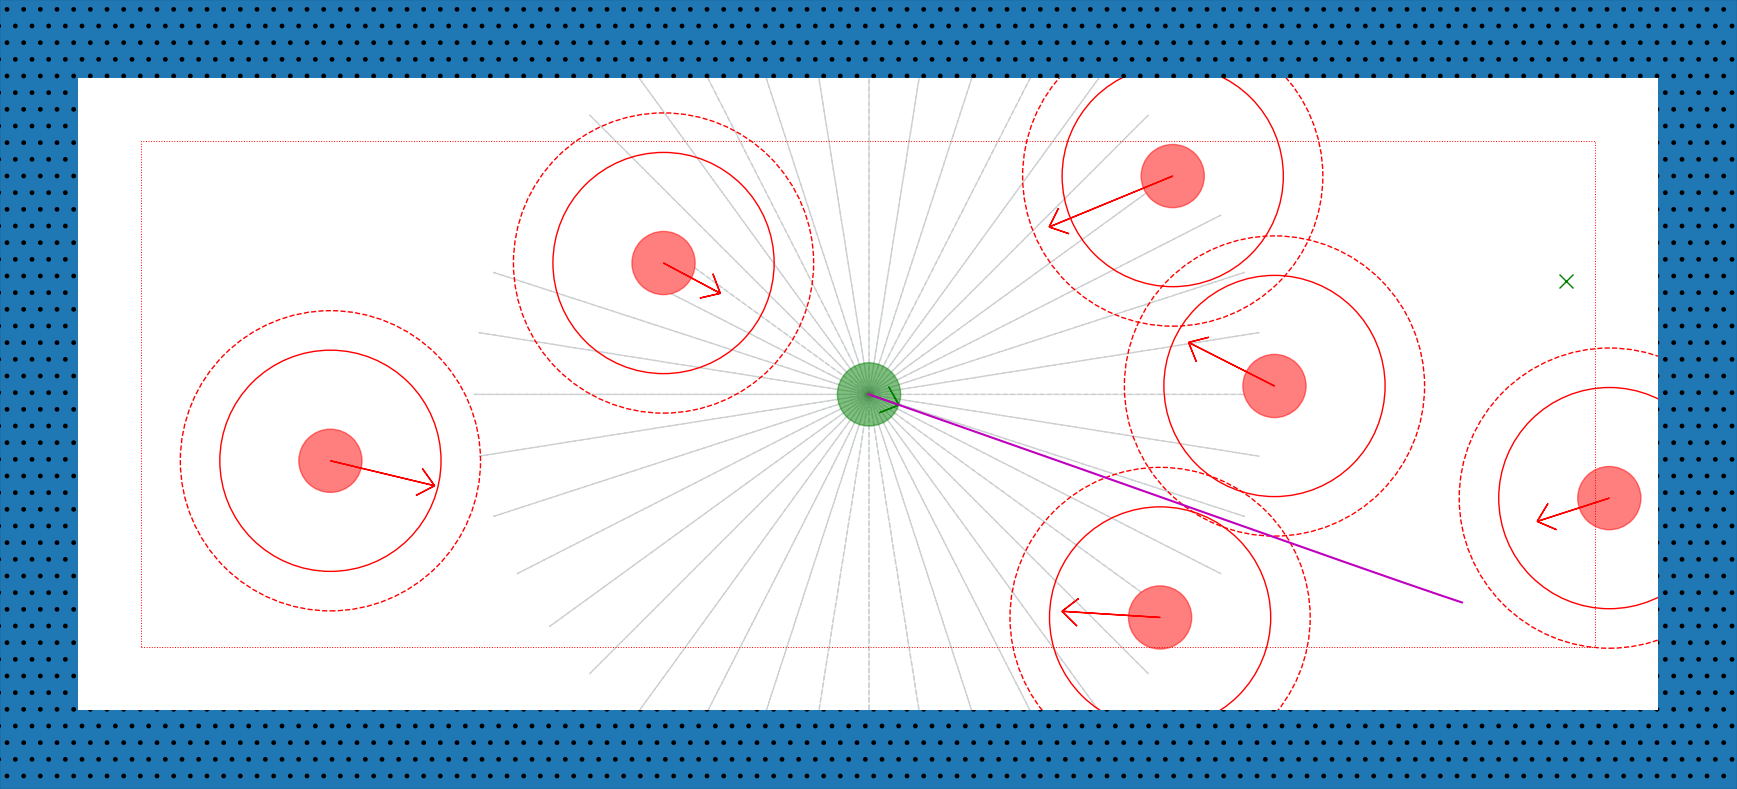
\includegraphics[width=0.48\textwidth]{figs/env.png}
    \caption{Crowd navigation environment with constant velocity crowd, using LiDAR observation (show in gray dashed line). The predicted trajectory from ProDMP is show in magenta.}
    \label{fig:env}
    \vspace{-2mm}
\end{figure}
The input can be arbitrarily complex including other social aspects from various sensors. The specific task we are interested in is local navigation with the main focus on behaving socially and avoiding moving and static obstacles in the environment. Exploring unknown environments or high-level logic on how to navigate between different areas of structured environments like buildings, are beyond the scope of this work. There are multiple options to define the MDP components for the task. For the observation we might consider positions and velocities or LiDAR rays, for actions space it is possible to choose between velocity or acceleration control. Similarly, the reward function can be set arbitrarily. We consider two main reward components: one for approaching and arriving at the goal and another for crowd proxemics and collisions
\begin{align*}
    r_{g} &= \begin{cases}
                10, & d_g < \tau_{\textsc{p}} \land \|\dot{\boldsymbol{p}}\| < a_{\textsc{max}}T, \\
                C_g \sign(p_g)p_g^2,
                 & \text{otherwise},
            \end{cases}\\
    r_{c_j} &= \begin{cases}
                0, & d_{c_i} > \tau_{\textsc{s}}, \\
                -10, & d_{c_i} < 2\tau_{\textsc{p}}, \\
                1 - \exp(C_c/d_{c_j}), & \text{otherwise},
             \end{cases}\\
    p_g&=d_{g,old}-d_g, \; d_g=\vert\vert\boldsymbol{p}-\boldsymbol{g}\vert\vert, \; d_{c_j}=\vert\vert \boldsymbol{p} - \boldsymbol{p}_{c_j}\vert\vert, \\
    \tau_g \: &\text{goal threshold distance},\; \tau_s\: \text{social threshold distance},\\ \tau_p \:&\text{physical threshold distance}.
\end{align*}
The transition function for the agent assumes an holonomic robot without the addition of disturbances. The transition function for other members of the crowd depends mainly on the algorithm used to model the crowd (constant velocity, ORCA \cite{berg_optimal_2011} or SFM \cite{helbing_social_1995}). The environment and the task configuration are discussed in more detail in a previous paper (reference omitted in submission version).
% In \cite{pikuli_navigating_2025} this environment and task configuration options are discussed in more detail.


\section{METHOD}

We use an episodic-RL approach in order to predict optimal trajectories to navigate the environment and apply MPC to minimize the distance from the reference trajectory while ensuring hard constraints. The two methods are independent from one another and it is part of the objective of the RL agent to learn a behaviour that best takes advantage of MPC.

\subsection{MPC for Navigation of a Holonomic Robot}\label{sec:mpc}

We assume an holonomic robot which implies straight forward dynamics from classical mechanics for the given agent position $\boldsymbol{p}_k$ at time $k$
\begin{align}
    \label{eq:dynamics}
    \boldsymbol{p}_{k+1} = \boldsymbol{p}_k + \dot{\boldsymbol{p}}_kT + \dfrac{1}{2}T^2\ddot{\boldsymbol{p}}_k &= \boldsymbol{p}_k + \dfrac{1}{2}\dot{\boldsymbol{p}}_kT + \dfrac{1}{2}T\dot{\boldsymbol{p}}_{k+1}\\
    \text{and} \quad \dot{\boldsymbol{p}}_{k+1} = \dot{\boldsymbol{p}}+T\ddot{\boldsymbol{p}} \;& \Leftrightarrow \; \ddot{\boldsymbol{p}}=\dfrac{\dot{\boldsymbol{p}}_{k+1}-\dot{\boldsymbol{p}}_k}{T}.\nonumber
\end{align}
To simplify the problem and reduce the numerical complexity (especially important for MPC), we apply velocity control. We further omit the step indexes when possible to avoid clutter. Iteratively we derive the transition matrix for a given horizon $N$ and current step $\boldsymbol{p}_0$ based on \Cref{eq:dynamics}
\begin{align}
    \label{eq:dynamics_horizon}
    &\quad\quad\quad\quad P=P_0+\dfrac{1}{2}T\dot{P}_0+M_{pv}\dot{P}, \quad (P=\boldsymbol{p}_{1:N}),\nonumber\\
    &P=\begin{bmatrix}P^{x\intercal} & P^{y\intercal}\end{bmatrix}^\intercal, \;\text{where} \;P^x=p^x_0+\dfrac{1}{2}T\dot{p}^x_0+M_{xv}\dot{P}^x,\nonumber\\
        &M_{xv} = \begin{bmatrix}\frac{1}{2} & 0 & \dots & 0 \\ 1 & \frac{1}{2} & \ddots & \vdots \\ \vdots & \ddots & \ddots & 0 \\ 1 & \dots & 1 & \frac{1}{2} \end{bmatrix}T, M_{pv}=\begin{bmatrix}
            M_{xv} & \boldsymbol{0} \\
            \boldsymbol{0} & M_{yv} \\
        \end{bmatrix},
\end{align}
where $P^x$ and $P^y$ are computed equivalently and $M_{xv}=M_{yv}\in\mathbb{R}^{N\times N}$. In the following, $x$ and $y$ will not be treated separately and we will concatenate appropriately to compute $P_0=\begin{bmatrix}
    p^x_0, & \dots & p^x_0, & p^y_0, & \dots & p^y_0
\end{bmatrix}\in\mathbb{R}^{2N}$, $\dot{P}_0\in\mathbb{R}^{2N}$, $M_{pv}\in\mathbb{R}^{2N\times 2N}$ and $\dot{P}\in\mathbb{R}^{2N}$.

Given our model we can define our cost function as the distance to a reference trajectory, $\frac{1}{2}\vert\vert P - P^{ref}\vert\vert$ (e.g. $P^{ref}$ is a straight line to the goal). This gives us a quadratic function to optimize after applying \Cref{eq:dynamics_horizon}
\begin{align*}
    &\min\limits_{\dot{P}}\frac{1}{2}\vert\vert P - P^{ref}\vert\vert \Leftrightarrow \min\limits_{\dot{P}}\frac{1}{2}\left(P-P^{ref}\right)^\intercal\left(P-P^{ref}\right) \nonumber\\
    \Leftrightarrow&\min\limits_{\dot{P}} \frac{1}{2}\dot{P}^\intercal\underbrace{M_{pv}^\intercal M_{pv}}_{\substack{=Q \\ \text{quadratic} \\ \text{term}}}\dot{P} +  \underbrace{\left(P_0-P^{ref}+ \frac{1}{2}T\dot{P}_0\right)^\intercal M_{pv}}_{=q \;\text{linear term}}\dot{P}.\nonumber
\end{align*}
Linear constraints can be arbitrarily added to this objective, see \Cref{tab:constraints}. For the crowd distance constraints we assume that the members of the crowd maintain the current velocity and increase the safety distance by the maximum distance in the error of the prediction. The maximum error will be lower than the distance covered during time-step $T$ with $\dot{\boldsymbol{p}}_{max}$, as represented in \Cref{fig:uncert}.
\begin{table}[ht]
    \centering
    \caption{Various constraints for MPC. $m_{i}$ and $b_{i}$ are the coefficients that define the edges ($y-m_ix-b_i<0$) of a polygon inscribed and approximating a circle implying a limited maximum value in all directions. $C$ is the number of members in the crowd and $p_{c_j,k}$ refers to crowd member $j$ at time-step $k$ and $d$ is the safety distance.}
    \label{tab:constraints}
    \begin{tabular}{ c | c }
    \hline
        Constraint & Equation\\
    \hline
        \makecell[c]{Passive \\ Safety} & \makecell[c]{
            explicitly set $\dot{p}^x_N=\dot{p}^y_N=0$ \\
            truncate $\dot{P}\in\mathbb{R}^{2(N-1)}$, $M_{pv}\in\mathbb{R}^{2N\times2(N-1)}$\\} \\
    \hline
        \thead{Velocity} & \makecell[c]{
                $M_{i}\dot{P} < B_i \quad \text{where}$ \\
                $M_{i}=\begin{bmatrix} -I_{N-1}m_i \vert I_{N-1}\end{bmatrix} \quad \text{and} \quad B_i=\begin{bmatrix}b_i, \dots b_i\end{bmatrix}^\intercal$
        }\\
    \hline
        \thead{Acceleration} & \makecell[l]{
            $M_{i}\begin{bmatrix} D & 0 \\ 0 & D\end{bmatrix}\dot{P}<B_i+\dfrac{M_{i}}{T}\begin{bmatrix} \dot{x}_0, 0, \dots \dot{y}_0, 0, \dots\end{bmatrix}^\intercal$\\
            $\text{where} \quad D =
            \begin{bmatrix*}[r]
                \tikzmarknode{top}{\boldsymbol{1}} & \tikzmarknode{upper}{\boldsymbol{0}} \\
                \tikzmarknode{top2}{\boldsymbol{-1}} & \tikzmarknode{bottom}{\boldsymbol{1}} \\
                \tikzmarknode{lower}{\boldsymbol{0}} & \tikzmarknode{bottom2}{\boldsymbol{-1}}
            \end{bmatrix*}\dfrac{1}{T}, D\in{N\times(N-1)}$
        }\\
    \hline
        \makecell[c]{Crowd \\ Distance \\ \cite{bohorquez_safe_2016}} & \makecell[c]{
            $\vert\vert \boldsymbol{p}_k - \boldsymbol{p}_{c_j,k}\vert\vert \geq d \quad \forall k\in\{1\dots N\}, j\in\{1\dots C\}$\\
            linearize $\hat{\boldsymbol{u}}^\intercal_c=\dfrac{\boldsymbol{p}-\boldsymbol{p}_c}{\vert\vert \boldsymbol{p}-\boldsymbol{p}_c\vert\vert}, \; \hat{\boldsymbol{u}}^\intercal_c(\boldsymbol{p}-\boldsymbol{p}_c)\geq d$\\
            $\xrightarrow{Eq. \ref{eq:dynamics_horizon}}\hat{U}_cM_{pv}\dot{P}\geq d-\hat{U}_c\left( P_0-P_c+\frac{1}{2}T\dot{P}_0\right)$\\
            with $\hat{U}_c=\begin{bmatrix}
                I_N\hat{\boldsymbol{u}}^x_{c,1:N} \vert I_N\hat{\boldsymbol{u}}^y_{c,1:N}
            \end{bmatrix}$
            } \\
    \hline
    \end{tabular}
\end{table}
\begin{tikzpicture}[remember picture, overlay]
    \draw [rounded corners]
        ([xshift=-15.6mm,yshift=-19mm]upper.center) --
        ([xshift=-7.2mm,yshift=-19mm]upper.center) --
        ([xshift=-7.2mm,yshift=-22.4mm]upper.center) --
        cycle;
\end{tikzpicture}
\begin{tikzpicture}[remember picture,overlay]
    \draw [rounded corners]
        ([xshift=-10 mm,yshift=-21.9mm]lower.center) --
        ([xshift=-1.8mm,yshift=-21.9mm]lower.center) --
        ([xshift=-10mm,yshift=-18.75mm]lower.center) --
        cycle;
\end{tikzpicture}
\begin{tikzpicture}[remember picture,overlay]
    \draw let \p1=($(top)-(bottom)$),\n1={atan2(\y1,\x1)} in node[xshift=-8.6mm,yshift=-20.5mm,rotate fit=\n1,fit=(bottom) (top),draw,rounded corners,inner sep=1.5pt]{};
\end{tikzpicture}
\begin{tikzpicture}[remember picture,overlay]
    \draw let \p1=($(top2)-(bottom2)$),\n1={atan2(\y1,\x1)} in node[xshift=-8.4mm,yshift=-20mm,rotate fit=\n1,fit=(bottom2) (top2),draw,rounded corners, inner xsep=1.5pt, inner ysep=0.5pt]{};
\end{tikzpicture}
\begin{figure}[ht]
    \centering
        \resizebox{8cm}{!}{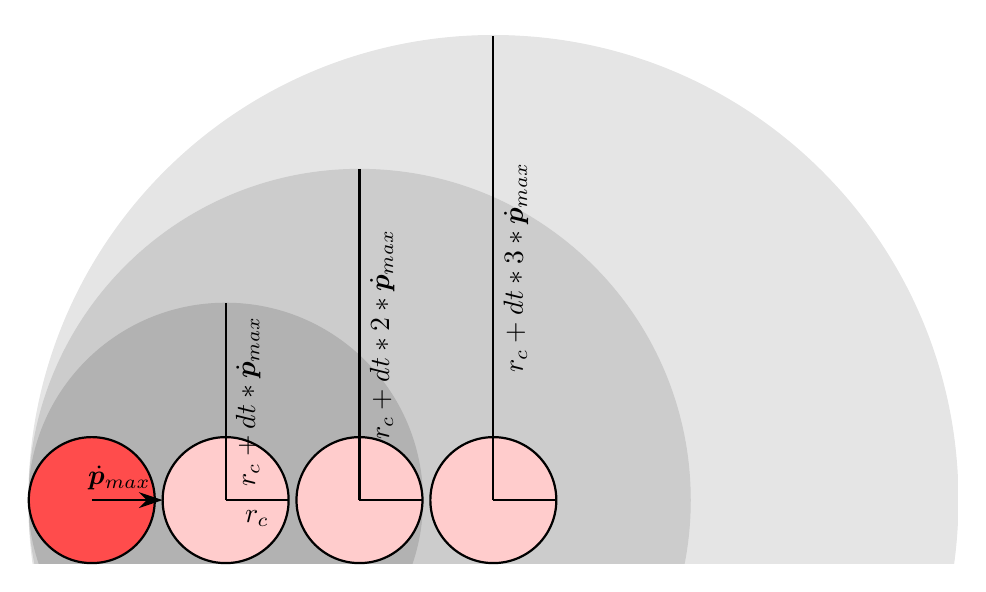
\begin{tikzpicture}
    % Define the centers and radii of the circles
    \coordinate (center1) at (0, 0);
    \filldraw[black, thick] (center1) circle(2pt);

    % Draw the first circle
    \begin{scope}
        \clip (-0.8,-0.81) rectangle (11,6);
        \draw[black!10, fill=black!10] ([xshift=5.1cm]center1) circle (5.9cm);
        \draw[black!20, fill=black!20] ([xshift=3.4cm]center1) circle (4.2cm);
        \draw[black!30, fill=black!30] ([xshift=1.7cm]center1) circle (2.5cm);
    \end{scope}
    \draw[black, thick, fill=red!70] (center1) circle (0.8cm);
    \draw[fill=red!20, thick] ([xshift=1.7cm]center1) circle (0.8cm);
    \draw[fill=red!20, thick] ([xshift=3.4cm]center1) circle (0.8cm);
    \draw[fill=red!20, thick] ([xshift=5.1cm]center1) circle (0.8cm);
    \draw[->, thick, -{Stealth[length=3mm, width=2mm]}]{(center1) -- ([xshift=0.9cm]center1) node[midway, above, xshift=-1mm] () {$\dot{\boldsymbol{p}}_{max}$}};
    \draw[thick]{
        ([xshift=1.7cm]center1) -- ([xshift=1.7cm, yshift=2.5cm]center1) node[midway, below, sloped] () {$r_c + dt * \dot{\boldsymbol{p}}_{max}$}
        ([xshift=1.7cm]center1) -- ([xshift=2.5cm]center1) node[midway, below] () {$r_c$}
    };
    \draw[thick]
        ([xshift=3.4cm]center1) -- ([xshift=3.4cm, yshift=4.2cm]center1) node[midway, below, sloped] () {$r_c + dt * 2 * \dot{\boldsymbol{p}}_{max}$}
        ([xshift=3.4cm]center1) -- ([xshift=4.2cm]center1)
    ;
    \draw[thick]
        ([xshift=5.1cm]center1) -- ([xshift=5.1cm, yshift=5.9cm]center1) node[midway, below, sloped] () {$r_c + dt * 3 * \dot{\boldsymbol{p}}_{max}$}
        ([xshift=5.1cm]center1) -- ([xshift=5.9cm]center1)
    ;
\end{tikzpicture}
}
    \caption{Uncertainty explodes for future predictions (shown here for three steps in the future).}
    \label{fig:uncert}
    \vspace{-0.5cm}
\end{figure}

\subsection{Learning Trajectories for Navigation}\label{sec:prodmp}

Episode-based RL can be more advantageous then step-based RL for specific tasks. In case of non-Markovian environments, environments where atomic steps are inaccessible or when learning temporal dependencies might be ineffective. Using motion primitives implies an episode representing a task. These approach to learning is motivated biologically as it has been well studied that certain movements are directly encoded in the nervous system. ML methods that learn motion primitives were proposed using the damped spring model \cite{Schaal2006,ijspeert_dynamical_2013} and more recently extended \cite{paraschos_probabilistic_2013,li_prodmps_2022}
\begin{equation}
    \label{eq:spring_model}
    \tau^2\ddot{y}=\alpha(\beta(g-y)-\tau\dot{y})-f,
\end{equation}
where $g$ represents the goal, $\alpha,\beta$ are constants and $f$ is the forcing term which we can define arbitrarily in order to execute desired trajectories. To cover the whole spectrum of desired movements, a weighted exponential basis functions scheme is used, motivated in \cite[Section 2.1]{Schaal2006}
\begin{equation}
    \label{eq:forcing_term}
    f(x)=x\dfrac{\sum_i\phi_i(x)w_i}{\sum_i\phi_i(x)} \quad \text{and} \quad \phi_i(x)=\exp{\left(\dfrac{-(x-\mu_i)^2}{2\sigma_i^2}\right)}.
\end{equation}
The advantage of using ProDMP \cite{li_prodmps_2022} is that it combines the strengths of DMPs (smooth replanning throughout the trajectory) and ProMPs (modelling of statistical properties) while requiring only one offline basis function  $\boldsymbol{\Phi}$ computation.
% instead of a costly online numerical integration as in DMP.
The replanning step is set arbitrarily and allows for better control as newer information becomes available to the policy. The Gaussian policy is used to sample a weight vector $\boldsymbol{w}\sim\mathcal{N}(\cdot\vert\boldsymbol{\mu}_{\boldsymbol{\theta}},\boldsymbol{\Sigma}_{\boldsymbol{\theta}})$ to parameterize the forcing function giving a trajectory $\boldsymbol{\lambda}=y_{1:N}$ using \Cref{eq:spring_model} and \Cref{eq:forcing_term}. In our case $y_k$ is not a scalar but a vector of two dimensions representing $x$ and $y$ coordinates on a 2D plane.

The policy is trained using TRPL \cite{otto_differentiable_2020}, a PG-based method that implements differentiable trust-regions to avoid policy collapse by limiting updates for a distance metric $D$ and tunable hyperparameter $\epsilon$
\begin{align}
    \label{eq:tr_rl}
    \boldsymbol{\theta}^\star&=\argmax_{\boldsymbol{\theta}}\mathbb{E}_{(s,a)\sim p_{\boldsymbol{\theta}}(\tau)}\left[Q^{\pi_{\boldsymbol{\theta}_{old}}}(s,a)\right], \nonumber \\
    &\text{s.t.}\quad D(\pi_{\boldsymbol{\theta}_{old}}, \pi_{\boldsymbol{\theta}}) < \epsilon,\quad \forall s\in\mathcal{S}.
\end{align}
TRPL introduces two advantages compared to PPO \cite{schulman2017ppo}: stability w.r.t. code-level optimizations \cite{Engstrom2020Implementation} and the capacity to constrain states individually. The objective in \Cref{eq:tr_rl} is simplified by using a Q-function, even though commonly a weighted (IS) advantage function is used. The conventional actions $a$ in this case are the weights to parameterize the ProDMP. TRPL has shown promising results in challenging tasks for learning ProDMP trajectories \cite{otto_deep_2023}.

We use a LiDAR representation for the obstacles around the agent and the relative position of the goal. In order to include information about the movement of the crowd, we use velocities along the LiDAR rays. To complete the observation, the 2D absolute velocity of the agent is given in order to be able to accelerate and decelerate accordingly. The architecture and decision making pipeline for the next action, given as velocity, is shown in \Cref{fig:policy}.
\begin{figure}[t]
    \centering
        \resizebox{8.4cm}{!}{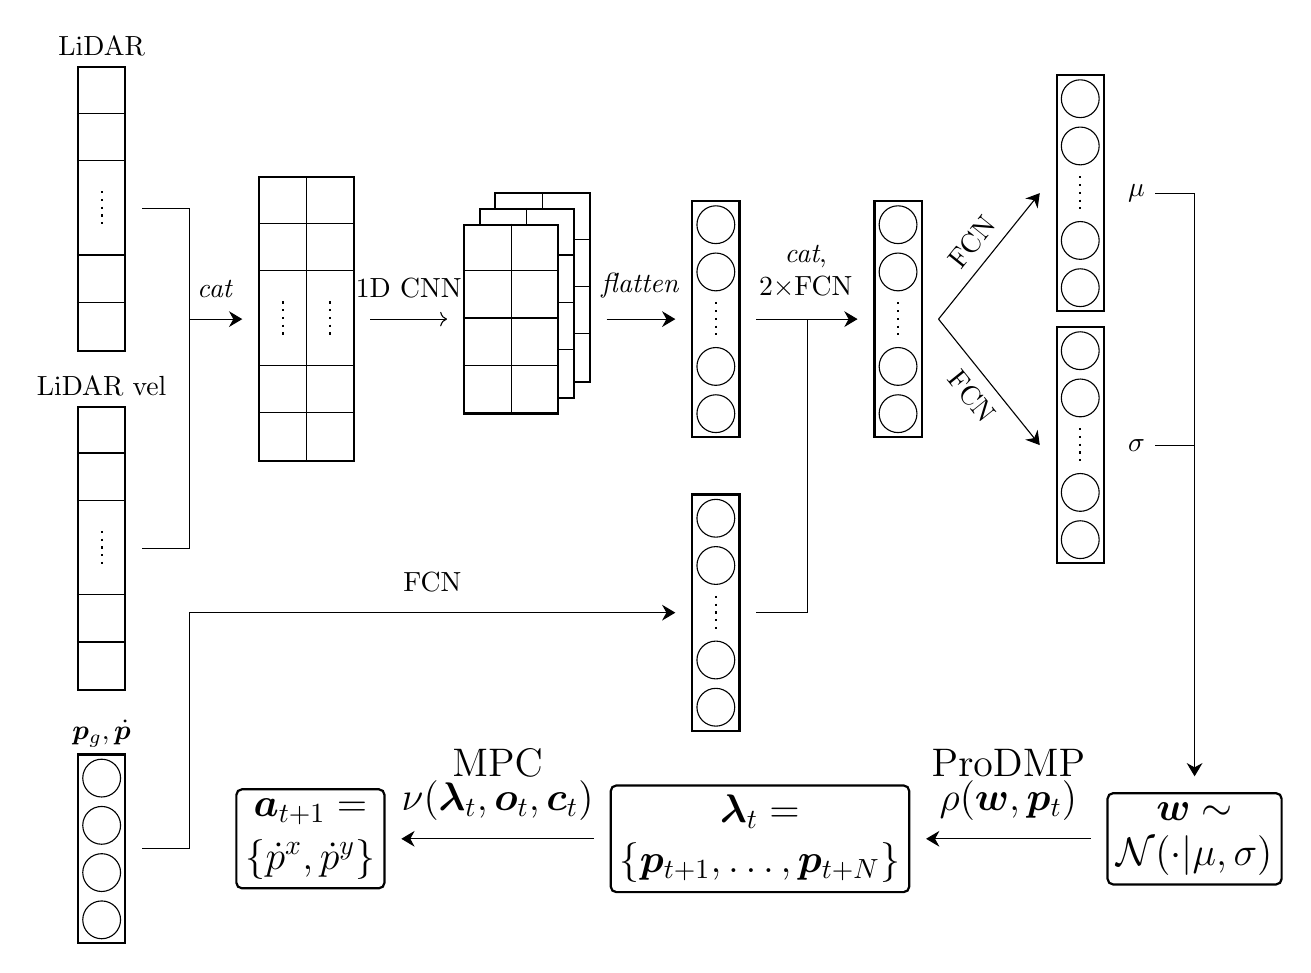
\begin{tikzpicture}[every node/.append style={align=center, thick}]
    \def\gridSize{6} % Number of squares per row and column
    \def\gridSizeIter{5} % Number of squares iteration, one less bc \gridSize - 1 not working in foreach
    \def\gridSizeCnn{4}
    \def\gridSizeCnnIter{3}
    \def\squareSize{0.6cm} % Size of each square

    % LiDAR obs
    \node[draw, minimum width=\squareSize, minimum height=\gridSize*\squareSize] (lidar) at (0, 0) {};
    \node (lidar_str) at ([yshift=2.5mm]lidar.north) {LiDAR};
    \foreach \i in {1,...,\gridSizeIter} {
      \ifnum \i = 3
            \draw[thick, dotted] ([yshift=-\i*\squareSize + 0.21cm]lidar.north) -- ([yshift=-\i*\squareSize - 0.21cm]lidar.north);
      \else
            \draw ([yshift=-\i*\squareSize]lidar.north west) -- ([yshift=-\i*\squareSize]lidar.north east);
       \fi
    }
    % LiDAR Vel obs
    \node[draw, minimum width=\squareSize, minimum height=\gridSize*\squareSize] (lidar_vel) at ([yshift=-2.5cm]lidar.south) {};
    \node (lidar_vel_str) at ([yshift=2.5mm]lidar_vel.north) {LiDAR vel};
    \foreach \i in {1,...,\gridSizeIter} {
      \ifnum \i = 3
            \draw[thick, dotted] ([yshift=-\i*\squareSize + 0.21cm]lidar_vel.north) -- ([yshift=-\i*\squareSize - 0.21cm]lidar_vel.north);
      \else
            \draw ([yshift=-\i*\squareSize]lidar_vel.north west) -- ([yshift=-\i*\squareSize]lidar_vel.north east);
       \fi
    }
    % Obs, goal position and velocity
    \node[draw, minimum width=\squareSize, minimum height=4*\squareSize] (obs) at ([yshift=-2cm]lidar_vel.south) {};
    \node (obs_str) at ([yshift=2.5mm]obs.north) {$\boldsymbol{p}_g, \dot{\boldsymbol{p}}$};
    \foreach \i in {0,...,3} {
       \draw ([yshift=-\i*\squareSize - \squareSize / 2 - 0.015cm]obs.north) circle (\squareSize / 2 - 0.06cm);
    }

    % Concatenate LiDAR and LiDAR Vel
    \node[draw, minimum width=2*\squareSize, minimum height=\gridSize*\squareSize] (lidar_cat) at ([xshift=2.6cm, yshift=-1.4cm]lidar) {};
    \foreach \i in {1,...,\gridSizeIter} {
      \ifnum \i = 3
            \draw[thick, dotted] ([yshift=-\i*\squareSize + 0.21cm, xshift=-\squareSize / 2]lidar_cat.north) -- ([yshift=-\i*\squareSize - 0.21cm, xshift=-\squareSize/2]lidar_cat.north);
            \draw[thick, dotted] ([yshift=-\i*\squareSize + 0.21cm, xshift=\squareSize / 2]lidar_cat.north) -- ([yshift=-\i*\squareSize - 0.21cm, xshift=\squareSize/2]lidar_cat.north);
      \else
            \draw ([yshift=-\i*\squareSize]lidar_cat.north west) -- ([yshift=-\i*\squareSize]lidar_cat.north east);
       \fi
    }
    \draw (lidar_cat.north) -- (lidar_cat.south);
    \draw ([xshift=0.2cm]lidar.east) -| ([xshift=0.8cm, yshift=-1.4cm]lidar.east);
    \draw ([xshift=0.2cm]lidar_vel.east) -| ([xshift=0.8cm, yshift=-1.4cm]lidar.east);
    \draw[->, -{Stealth[width=2mm]}] ([xshift=0.8cm, yshift=-1.4cm]lidar.east) -- ([xshift=-0.2cm]lidar_cat.west) node[midway, above, yshift=4pt] () {\textit{cat}};

    % CNN
    \node[draw, fill=white, minimum width=2*\squareSize, minimum height=\gridSizeCnn*\squareSize] (cnn_lidar) at ([xshift=3cm,yshift=0.4cm]lidar_cat) {};
        \foreach \i in {1,...,\gridSizeCnnIter} {
            \draw ([yshift=-\i*\squareSize]cnn_lidar.north west) -- ([yshift=-\i*\squareSize]cnn_lidar.north east);
        }
        \draw (cnn_lidar.north) -- (cnn_lidar.south);

    \node[draw, fill=white, minimum width=2*\squareSize, minimum height=\gridSizeCnn*\squareSize] (cnn_lidar) at ([xshift=2.8cm,yshift=0.2cm]lidar_cat) {};
        \foreach \i in {1,...,\gridSizeCnnIter} {
            \draw ([yshift=-\i*\squareSize]cnn_lidar.north west) -- ([yshift=-\i*\squareSize]cnn_lidar.north east);
        }
        \draw (cnn_lidar.north) -- (cnn_lidar.south);
    \node[draw, fill=white, minimum width=2*\squareSize, minimum height=\gridSizeCnn*\squareSize] (cnn_lidar) at ([xshift=2.6cm]lidar_cat) {};
        \foreach \i in {1,...,\gridSizeCnnIter} {
            \draw ([yshift=-\i*\squareSize]cnn_lidar.north west) -- ([yshift=-\i*\squareSize]cnn_lidar.north east);
        }
        \draw (cnn_lidar.north) -- (cnn_lidar.south);
    \draw [->] ([xshift=0.2cm]lidar_cat.east) -- ([xshift=-0.2cm]cnn_lidar.west) node[midway, above, yshift=4pt] () {1D CNN};

    % MLP for obs
    \node[draw, minimum width=\squareSize, minimum height=5*\squareSize] (obs_mlp) at ([yshift=3cm, xshift=7.8cm]obs) {};
    \foreach \i in {0,...,4} {
        \ifnum \i = 2
            \draw[thick, dotted] ([yshift=-\i*\squareSize - \squareSize / 2  + 0.2cm]obs_mlp.north) -- ([yshift=-\i*\squareSize - \squareSize / 2  - 0.22cm]obs_mlp.north);
        \else
            \draw ([yshift=-\i*\squareSize - \squareSize / 2 - 0.015cm]obs_mlp.north) circle (\squareSize / 2 - 0.06cm);
        \fi
    }
    \draw ([xshift=0.2cm]obs.east) -| ([xshift=0.8cm, yshift=3cm]obs.east);
    \draw [->, -{Stealth[width=2mm]}] ([xshift=0.8cm, yshift=3cm]obs.east) -- ([xshift=-0.2cm]obs_mlp.west)  node[midway, above, yshift=4pt] () {FCN};

    % Flatten
    \node[draw, minimum width=\squareSize, minimum height=5*\squareSize] (flat_lidar) at ([xshift=2.6cm]cnn_lidar) {};
    \foreach \i in {0,...,4} {
        \ifnum \i = 2
            \draw[thick, dotted] ([yshift=-\i*\squareSize - \squareSize / 2  + 0.2cm]flat_lidar.north) -- ([yshift=-\i*\squareSize - \squareSize / 2  - 0.22cm]flat_lidar.north);
        \else
            \draw ([yshift=-\i*\squareSize - \squareSize / 2 - 0.015cm]flat_lidar.north) circle (\squareSize / 2 - 0.06cm);
        \fi
    }
    \draw [->, -{Stealth[width=2mm]}] ([xshift=0.6cm]cnn_lidar.east) -- ([xshift=-0.2cm]flat_lidar.west)  node[midway, above, yshift=4pt] () {\textit{flatten}};

    \draw ([xshift=0.2cm]flat_lidar.east) -- ([xshift=0.85cm]flat_lidar.east);
    \draw ([xshift=0.2cm]obs_mlp.east) -| ([xshift=0.85cm]flat_lidar.east);

    % FCN after cat
    \node[draw, minimum width=\squareSize, minimum height=5*\squareSize] (mlp_cat_0) at ([xshift=2cm]flat_lidar.east) {};
    \foreach \i in {0,...,4} {
        \ifnum \i = 2
            \draw[thick, dotted] ([yshift=-\i*\squareSize - \squareSize / 2 + 0.2cm]mlp_cat_0.north) -- ([yshift=-\i*\squareSize - \squareSize / 2  - 0.22cm]mlp_cat_0.north);
        \else
            \draw ([yshift=-\i*\squareSize - \squareSize / 2 - 0.015cm]mlp_cat_0.north) circle (\squareSize / 2 - 0.06cm);
        \fi
    }
    \draw [->, -{Stealth[width=2mm]}] ([xshift=0.85cm]flat_lidar.east) -- ([xshift=-0.2cm]mlp_cat_0.west) node[midway, above, xshift=-0.34cm, yshift=4pt] () {\textit{cat},\\ 2$\times$FCN};

    % Mean
    \node[draw, minimum width=\squareSize, minimum height=5*\squareSize] (mlp_mean) at ([yshift=-1.6cm, xshift=2cm]mlp_cat_0.east) {};
    \node (mlp_mean_str) at ([xshift=0.4cm]mlp_mean.east) {$\sigma$};
    \foreach \i in {0,...,4} {
        \ifnum \i = 2
            \draw[thick, dotted] ([yshift=-\i*\squareSize - \squareSize / 2  + 0.2cm]mlp_mean.north) -- ([yshift=-\i*\squareSize - \squareSize / 2  - 0.22cm]mlp_mean.north);
        \else
            \draw ([yshift=-\i*\squareSize - \squareSize / 2 - 0.015cm]mlp_mean.north) circle (\squareSize / 2 - 0.06cm);
        \fi
    }
    \draw [->, -{Stealth[width=2mm]}] ([xshift=0.2cm]mlp_cat_0.east) -- ([xshift=-0.2cm]mlp_mean.west)  node[midway, below, yshift=-1pt, sloped] () {FCN};
    % STD
    \node[draw, minimum width=\squareSize, minimum height=5*\squareSize] (mlp_std) at ([yshift=1.6cm, xshift=2cm]mlp_cat_0.east) {};
    \node (mlp_std_str) at ([xshift=0.4cm]mlp_std.east) {$\mu$};
    \foreach \i in {0,...,4} {
        \ifnum \i = 2
            \draw[thick, dotted] ([yshift=-\i*\squareSize - \squareSize / 2  + 0.2cm]mlp_std.north) -- ([yshift=-\i*\squareSize - \squareSize / 2  - 0.22cm]mlp_std.north);
        \else
            \draw ([yshift=-\i*\squareSize - \squareSize / 2 - 0.015cm]mlp_std.north) circle (\squareSize / 2 - 0.06cm);
        \fi
    }
    \draw [->, -{Stealth[width=2mm]}] ([xshift=0.2cm]mlp_cat_0.east) -- ([xshift=-0.2cm]mlp_std.west)  node[midway, above, yshift=1pt, sloped] () {FCN};

    % Weight sampling
    \draw (mlp_std_str) -| ([xshift=0.5cm]mlp_mean_str.east);
    \draw (mlp_mean_str) -- ([xshift=0.5cm]mlp_mean_str.east);
    \node[rectangle, draw=black, rounded corners=2pt] (weights) at ([xshift=0.5cm, yshift=-5cm]mlp_mean_str.east) {\Large$\boldsymbol{w}\sim$ \\[1ex] \Large$\mathcal{N}(\cdot\vert\mu,\sigma)$};
    \draw [->, -{Stealth[width=2mm]}] ([xshift=0.5cm]mlp_mean_str.east) -- ([yshift=0.2cm]weights.north);
    \node[rectangle, draw=black, rounded corners=2pt] (traj) at ([xshift=-4.4cm]weights.west) {\Large$\boldsymbol{\lambda}_t=$\\[1ex] \Large$\{\boldsymbol{p}_{t+1},\dots,\boldsymbol{p}_{t+N}\}$};
    \draw [->, -{Stealth[width=2mm]}] ([xshift=-0.2cm]weights.west) -- ([xshift=0.2cm]traj.east) node[midway, above, yshift=3pt] () {\Large ProDMP \\ \Large $\rho(\boldsymbol{w}, \boldsymbol{p}_t)$};
    \node[rectangle, draw=black, rounded corners=2pt] (action) at ([xshift=-3.8cm]traj.west) {\Large$\boldsymbol{a}_{t+1}=$\\[1ex] \Large$\{\dot{p}^x,\dot{p}^y\}$};
    \draw [->, -{Stealth[width=2mm]}] ([xshift=-0.2cm]traj.west) -- ([xshift=0.2cm]action.east) node[midway, above, yshift=3pt] () {\Large MPC \\ \Large $\nu(\boldsymbol{\lambda}_t,\boldsymbol{o}_t,\boldsymbol{c}_t)$};

\end{tikzpicture}
}
    \caption{Policy architecture. Where $\boldsymbol{o}_t$ relates to the current observation of the environment and $\boldsymbol{c}_t$ the resulting constraints.}
    \label{fig:policy}
\end{figure}

\subsection{MPC as Safety Filter for Episode-based RL}\label{sec:const}

We propose to combine both approaches by setting the reference trajectory in the MPC objective to the prediction from the ProDMP TRPL policy $P^{ref}\coloneqq \boldsymbol{\lambda}$. The length for the prediction must be longer than the MPC horizon. Moreover, it is important to set the rate $r$ at which the policy replans the path. A high replanning period will results in worse predictions for steps far in the future. A short horizon will increase computational cost while not introducing any jerky behaviour thanks to the properties of ProDMP. The reference trajectory is truncated for MPC and optimization is executed in a closed-loop control manner until replanning is reengaged. In Algorithm \ref{algo:main}, the two stages of the policy are shown. In lines 3-6 the new trajectory is computed, in line 7 the reference trajectory for the MPC objective is set. In lines 8 and 9 the necessary matrices, vectors are updated in order to run the QP optimization (line 10) with constraints.

While learning should allow for a proper symbiotic relation between the two components, various considerations can accelerate the learning process. This entails mainly hyperparameters like the \textit{stability coefficient} for MPC in order to encourage smooth control, the horizon $N$ for MPC and the \textit{goal scale} for ProDMP to set a suitable length for the trajectories learned. This is further discussed in \Cref{sec:eval}.
\begin{algorithm}
\caption{Inference of ProDMP MPC}\label{algo:main}
    \KwData{Policy $\boldsymbol{\theta}$, ProDMP ($\boldsymbol{\Phi}$, $M$, $r$),\\ \hspace{8.4mm} MPC ($N, M_{pv}, M_i, b_i, d$), env $e$}
$s_t \gets e.init()$\;
\While{$t < e.max\_steps$}{
    \If{$t \mod r = 0$ }{
        $\boldsymbol{w}_t \gets \mu_{\boldsymbol{\theta}}(s_t)$\;
        $\boldsymbol{\lambda}_{t:t+M} \gets \boldsymbol{\Phi}\boldsymbol{w}_t$ \Comment*[r]{Eq. \ref{eq:spring_model}, \ref{eq:forcing_term}}
    }
    $P^{ref} \gets \boldsymbol{\lambda}_{t:t+N}$\;
    \tcp{Matrices \& crowd prediction}
    $\{Q, q, \hat{U}_c,P_c\} \gets mat(s_t,M_{pv},M_i,b_i,P^{ref},d) $\;
    \tcp{Constraints as in \Cref{tab:constraints}}
    $\boldsymbol{c_t} \gets const(s_t,Q,q,M_{pv},M_i,b_i,d,\hat{U}_c,P_c) $\;
    $\dot{P}^\star \gets \argmin_{\dot{P}}\vert\vert P - P^{ref}\vert\vert$ s.t. $c_{t,i} \:\forall i$\;
    $a_t \gets \dot{P}^\star_1$ \Comment*[r]{Feedback control}
    $s_t, r_t, done_t \gets e.step(a_t)$\;
}
\end{algorithm}

\section{EVALUATION}\label{sec:eval}

We evaluate our approach in three main perspectives: efficiency, safety and FRP. At the same time we compare two aspects: the improvements brought to MPC and RL when combining the two and the difference in performance to the state of the art \cite{everett_collision_2021}. For the latter an evaluation benchmark is already implemented in \verb!gym-collision-avoidance! (GCA) \footnote{\url{link/to/gca_environment}}. The general setup involves an agent or multiple agents controlled by the same or different policies with each a goal position. No static obstacles or walls are considered in this environment, however the observation remains the same since we use LiDAR. During training and testing we make use of a crowd modeling algorithm ORCA \cite{berg_optimal_2011}. As metrics we use the \textit{return}, \textit{time to goal} (TTG) and \textit{success rate} (reaching the goal) for efficiency or performance. Safety is evaluated based on \textit{collision rate} and for the gravity of the collision we use \textit{collision speed}, \textit{collision agent speed} and \textit{maximum collision intersection} (this is the maximal overlap between colliding agents if they would go through one another, a high percentage indicates a greater overlap and a more direct collision). FRP is prominent with classical constraint-based approaches, so we evaluate the advantages against MPC. There is no well-established metric to quantify the problem, we propose to use the number of times that the QP-solver fails to find a solution given constraints. In this case the last computed braking trajectory is applied which means that the robot will potentially stop.
% using a threshold time coefficient during which the agent should not freeze, move further from the goal or oscillate `indecisively' similarly to \cite{sathyamoorthy_frozone_2020}.

ProDMP was trained using the \verb!CrowdNavigation!\footnote{\url{link/to/environment}} environment. We use a time-step $T$ of $0.1s$, replanning $r$ every $2$ steps ($0.2s$) and MPC horizon $N$ of $20$ ($2s$). MPC includes in its objective a stability term in order to encourage smoother control. This is an especially important factor when implementing the intrinsic reward
\begin{align*}
    r_i = \alpha\sum_{t}^{t+r}\left\vert\left\vert P_t - P^{ref}_t\right\vert\right\vert,
\end{align*}
as the MPC behaviour becomes unpredictable for RL when the term is omitted. There are limitations to the effect of the intrinsic component for highly jerky control from MPC. This can happen when considering uncertainty in the crowd prediction. In order to ensure passive safety, the crowd distance $d$ is augmented for future positions by the maximum error in distance prediction, as discussed in \Cref{sec:mpc} and shown in \Cref{fig:uncert}. With this conservative constraint the FRP becomes more noticeable. We use the QP-solver \cite{goulart_clarabel_2024} with tolerance parameters of $10^{-5}$. Moreover, crowd-distance, velocity and acceleration constraints are removed when possible based on distance and velocity in order to lower the computational footprint. Further implementations details can be found for all components \verb!MPCCrowdNav!\footnote{\url{link/to/mpc}}, \verb!TrustRegionProjectionLayers!\footnote{\url{link/to/rl_algorithm}}.
% Further implementations details can be found for all components \footnote{https://github.com/dhimiter49/gym-collision-avoidance/tree/prodmp_policy} \textbf{CrowdNavigation}{https://github.com/dhimiter49/fancy_gym_crowd/tree/crowd_nav} \textbf{MPCCrowdNav}\footnote{\url{https://github.com/dhimiter49/mpc_crowd_nav}}, \textbf{TrustRegionProjections}\footnote{\url{https://github.com/dhimiter49/TrustRegionProjections}}.

\subsection{Constant Velocity Crowd}

In this environment, shown in \Cref{fig:env}, the prediction of the future position of the crowd is perfect, which should give the best performance for MPC. From evaluation, the analysis is more complex. In \Cref{tab:const}, we see a collection of results for different algorithms. MPC is able to consistently go faster to the goal due to its objective to do so on a straight path with $\dot{\boldsymbol{p}}_{max}$. This results in low TTG but may also reduce the success rate because it ignores the crowd and the optimal path to take relative to the crowd. This is the reason why combining MPC with a learned RL reference trajectory results in a higher success rate. While a lower TTG means a higher return, at the same time ignoring a comfortable distance to the crowd penalises MPC agents and increasing the distance constraint in order to optimize this component of the reward would introduce a lot of inefficiency w.r.t. reaching the goal quickly. As expected, pure RL methods achieve high return, especially ProDMP while SAC maintains a high collision rate reducing the final return. As a reminder the return is an arbitrary metric, by lowering the coefficient for the goal completion $C_g$ it is possible to have a higher return for ProDMP MPC approaches compared to MPC, and similarly by increasing the penalty for collisions (default is $-10$) it is possible to have a higher return for ProDMP MPC when compared to SAC and ProDMP.
\begin{table*}[ht]
    \centering
    \caption{Algorithm comparison for constant crowd environment.}
    \label{tab:const}
    \begin{tabular}{ | c | c | c | c | c | c | c | c | c |   }
    \hline
        \makecell{Metrics} & \makecell{SAC} & \makecell{ProDMP} & \makecell{MPC \\ $N=10$} & \makecell{MPC \\ $N=20$} & \makecell{MPC SH \\ $N=20$} & \makecell{ProDMP MPC \\ $N=20$}  & \makecell{ProDMP MPC \\ $N=20$, SH} \\
    \hline
        return $\uparrow$ & \textcolor{lightgreen}{\textbf{8.33}} $\pm$ 0.19  & \textcolor{mygreen}{\textbf{10.19}}  $\pm$ 0.11 & \textcolor{lightgreen}{\textbf{8.51}} & \textcolor{lightgreen}{\textbf{8.32}}& \textcolor{mygreen}{\textbf{8.66}} & 7.94 $\pm$ 0.11 & 7.99 $\pm$ 0.12 \\
        TTG $\downarrow$ (s) & 7.34 $\pm$ 0.05 & 7.19 $\pm$ 0.07  & \textcolor{mygreen}{\textbf{6.37}} & \textcolor{mygreen}{\textbf{6.43}} & \textcolor{mygreen}{\textbf{6.36}} & 7.76 $\pm$ 0.07  & 7.76 $\pm$ 0.07  \\
        success $\uparrow$ (\%) & 92.14 $\pm$ 0.49  & \textcolor{lightgreen}{\textbf{95.38}} $\pm$ 0.61  & 93.8  & 93.5  & 93.9  & \textcolor{mygreen}{\textbf{96.22}} $\pm$ 0.2  & \textcolor{mygreen}{\textbf{96.56}} $\pm$ 0.21  \\
    \hline
        col. $\downarrow$ (\%) & \textcolor{myred}{\textbf{7.3}} $\pm$ 0.82  & \textcolor{myred}{\textbf{4.42}} $\pm$ 0.67  & 1.0  & 0.5   & \textcolor{mygreen}{\textbf{0.3}}  & 0.6 $\pm$ 0.23  & \textcolor{mygreen}{\textbf{0.26}} $\pm$ 0.08  \\
        $\vert\vert\dot{p}-\dot{p}_c\vert\vert\downarrow$ (m/s) & \textcolor{myred}{\textbf{1.7}} $\pm$ 0.07  & \textcolor{myred}{\textbf{1.39}} $\pm$ 0.08  & 1.19  & \textcolor{mygreen}{\textbf{0.98}}  & 1.02  & 1.16 $\pm$ 0.04  & 1.07 $\pm$ 0.13 \\
        $\vert\vert\dot{p}\vert\vert\downarrow$ (m/s) & \textcolor{myred}{\textbf{0.94}} $\pm$ 0.01  & \textcolor{myred}{\textbf{0.95}} $\pm$ 0.01  & \textcolor{mygreen}{\textbf{0.0}}  & \textcolor{mygreen}{\textbf{0.0}}  & \textcolor{mygreen}{\textbf{0.0}}  & \textcolor{mygreen}{\textbf{0.0}} $\pm$ 0.0  & \textcolor{mygreen}{\textbf{0.0}} $\pm$ 0.0  \\
        col. area $\downarrow$ (\%) &\textcolor{mygreen}{\textbf{22.0}} $\pm$ 3.09  & \textcolor{mygreen}{\textbf{19.28}} $\pm$ 3.86  & 61.57  & 77.6  & 36.84  & 63.93 $\pm$ 16.37  &  58.64 $\pm$ 12.49  \\
    \hline
        braking $\downarrow$ (\%) & - & - & 2.9 & 8.5 & \textcolor{mygreen}{\textbf{0.3}} & 1.72 $\pm$ 0.31 & \textcolor{mygreen}{\textbf{0.26}} $\pm$ 0.08 \\
    \hline
    \end{tabular}
    \vspace{-0.5cm}
\end{table*}

Because of the perfect prediction of the crowd, ProDMP MPC does not introduce a clear advantage in collision rate and collision speed. Unsurprisingly, both methods perform much better than RL methods on this regard. Collisions still happen because of the high density of the crowd, which results in the agent finding itself in a situation where it cannot escape a collision. Some trained seeds of ProDMP MPC are able to avoid all collisions, however this comes at the cost of efficiency. In general, the collision speed and area of intersection are highly noisy, but the higher collision speed for SAC and ProDMP is notable. On the contrary, the collision intersection area is lower for these methods as the policy evades the collision until the last moment while MPC based approaches only require stopping before the collision happens without further consideration on severity. At the same time, some metrics might be inversely correlated, e.g. a lower collision rate might also indicate that the remaining collisions will be more severe thus less avoidable and analogously for TTG and success rate. The TTG will be lower for easier scenarios while lowering the success rate when failing more complicated scenarios.

Finally, its is clear that the number of braking instances reduces with a lower horizon and when using ProDMP. Going from horizon 20 to 10 reduces the braking trajectories by almost 6\% whereas using learned trajectories by almost 7\%. By far the most effective way of avoiding braking trajectories is to reduce the horizon. This is intuitive as lowering the horizon can drastically lower the number of constraints. We dynamically change the horizon while running MPC in cases where the QP-solver does not find a solution. Up to 3 shorter horizons are executed by reducing in half (by default it is shortened from 20 to 10 to 5 to 3). For a high enough deceleration speed the shortened horizon introduces no problems for passive safety. Using this technique has altogether a positive effects on all metrics. It is important to mention that, simply using a shorter horizon by default will have a negative effect on the ability of MPC to avoid future collisions. Based on the experiments on the constant crowd we set a default MPC horizon of 20 (2s). Longer trajectories of 30 and 40 steps introduced no notable advantage in our environment setup.

\subsection{ORCA crowd}

By using ORCA \cite{berg_optimal_2011} the crowd prediction cannot be perfect as the crowd will accelerate and decelerate towards the goal while avoiding collisions. In order to make the task more difficult for the agent, members modeled though ORCA will take in consideration only a fraction of the actual physical space the agent occupies. This means that the major part of the collision avoidance task has to be undertaken by the agent itself. In practice the radius of the agents is one forth of its real size from the perspective of ORCA.

Because of the uncertainty in the position of the crowd, MPC performs quite poorly and it will often engage in braking trajectories that lead to crashes as the ORCA policy will not avoid the entire physical space of the agent, see \Cref{tab:orca}. The gain in performance is clear when dropping uncertainty and assuming constant velocity, however this has a negative effect on safety while ProDMP remains more performant overall. In this case collisions increase even more and of course passive safety is violated. Using ProDMP with MPC introduces some clear advantages as the percentage of braking trajectory severely decreases. As mentioned before training ProDMP with crowd uncertainty proved to be too difficult as the control that MPC applies on top of the ProDMP trajectory gets very unsmooth. The ProDMP MPC agents shown in \Cref{tab:orca} where trained without crowd uncertainty which violates passive safety, however greatly reduces collision rate and has seemingly no negative effect on collision speed. Adding crowd uncertainty almost halves the success rate while doubling crash percentage.
\begin{table*}[ht]
    \centering
    \caption{Algorithm comparison for crowd running with ORCA.}
    \label{tab:orca}
    \begin{tabular}{ | c | c | c | c | c | c | c | c | c | c | c | }
    \hline
        \makecell{Metrics}& \makecell{MPC \\ uncert} & \makecell{MPC SH \\ uncert} & \makecell{MPC SH} & \makecell{SAC} & \makecell{ProDMP} & \makecell{ProDMP MPC} &  \makecell{ProDMP MPC \\ SH} & \makecell{ProDMP MPC \\ uncert, SH} \\
    \hline
        return $\uparrow$ & -5.4  & 1.75  & 3.65 & 1.56 $\pm$ 0.52 & \textcolor{mygreen}{\textbf{6.25}} $\pm$ 0.47 & \textcolor{lightgreen}{\textbf{4.94}} $\pm$ 0.16 & \textcolor{mygreen}{\textbf{5.03}} $\pm$ 0.16 & 2.71 $\pm$ 0.39\\
        TTG $\downarrow$ (s) & 7.91   & 7.73 & \textcolor{lightgreen}{\textbf{7.46}} & \textcolor{mygreen}{\textbf{6.44}} $\pm$ 0.29 & 8.3 $\pm$ 0.07 & 8.72 $\pm$ 0.07  & 8.73 $\pm$ 0.07  & 8.71 $\pm$ 0.16 \\
        success $\uparrow$ (\%) & \textcolor{myred}{\textbf{30.3}} & \textcolor{lightgreen}{\textbf{53.5}}   & \textcolor{mygreen}{\textbf{72.8}} & 39.3 $\pm$ 1.94 & \textcolor{mygreen}{\textbf{63.54}} $\pm$ 2.09 & \textcolor{mygreen}{\textbf{61.58}} $\pm$ 3.09  & \textcolor{mygreen}{\textbf{62.0}} $\pm$ 3.14  & \textcolor{myred}{\textbf{32.82}} $\pm$ 1.08 \\
    \hline
        col. $\downarrow$ (\%) & \textcolor{myred}{\textbf{22.1}} & \textcolor{myred}{\textbf{16.9}}   & \textcolor{myred}{\textbf{23.8}} & \textcolor{myred}{\textbf{19.6}} $\pm$ 4.38 & \textcolor{myred}{\textbf{12.86}} $\pm$ 1.47 & \textcolor{lightgreen}{\textbf{2.08}} $\pm$ 0.38  & \textcolor{mygreen}{\textbf{1.66}} $\pm$ 0.33  & \textcolor{lightgreen}{\textbf{3.32}} $\pm$ 0.43 \\
        $\vert\vert\dot{p}-\dot{p}_c\vert\vert\downarrow$ (m/s) & 1.27 & 1.26 & \textcolor{mygreen}{\textbf{1.04}} & \textcolor{myred}{\textbf{1.74}} $\pm$ 0.08 & \textcolor{mygreen}{\textbf{1.06}} $\pm$ 0.04 & 1.15 $\pm$ 0.09  & \textcolor{mygreen}{\textbf{1.1}} $\pm$ 0.08  & 1.2 $\pm$ 0.02 \\
        $\vert\vert\dot{p}\vert\vert$ $\downarrow$ (m/s) & \textcolor{mygreen}{\textbf{0.0}} & \textcolor{mygreen}{\textbf{0.0}} & \textcolor{myred}{\textbf{0.64}} & \textcolor{myred}{\textbf{0.94}} $\pm$ 0.02 & \textcolor{myred}{\textbf{0.98}} $\pm$ 0.01 & \textcolor{myred}{\textbf{0.69}} $\pm$ 0.05  & \textcolor{myred}{\textbf{0.67}} $\pm$ 0.04  & \textcolor{mygreen}{\textbf{0.0}} $\pm$ 0.0 \\
        col. area $\downarrow$ (m$^2$) & 5.86 & 6.38 & 5.53 & 7.89 $\pm$ 0.9 & 7.58 $\pm$ 0.83 & 3.83 $\pm$ 0.69  & \textcolor{mygreen}{\textbf{2.56}} $\pm$ 1.71  & 6.96 $\pm$ 0.36 \\
    \hline
        braking $\downarrow$ (\%)& \textcolor{myred}{\textbf{162.2}} & 20.6 & 12.5 & - & - & 10.28 $\pm$ 0.92  & \textcolor{mygreen}{\textbf{0.74}} $\pm$ 0.23  & 4.22 $\pm$ 0.48 \\
    \hline
    \end{tabular}

    \vspace{2mm}

    \begin{tabular}{ | c | c | c | c | c | c | c | }
    \hline
        \makecell{Metrics} & \makecell{MPC \\ uncert \\ $N=10$} & \makecell{MPC SH \\ uncert \\ $N=10$} & \makecell{MPC \\ uncert \\ $N=5$} & \makecell{ProDMP MPC \\ uncert, SH \\ $N=20$} & \makecell{ProDMP MPC \\ uncert, SH \\ $N=10$} & \makecell{ProDMP MPC \\ uncert, SH \\ $N=5$} \\
    \hline
        return $\uparrow$ & -1.79 & 1.2 & -0.82 & 3.19 $\pm$ 0.38 & 4.31 $\pm$ 0.37 & 4.56 $\pm$ 0.22 \\
        TTG $\downarrow$ (s) & 7.75 & 7.64 & 7.68 & 8.54 $\pm$ 0.07 & 8.38 $\pm$ 0.08 & 8.35 $\pm$ 0.13 \\
        success $\uparrow$ (\%) & 47.9 & 57.7 & 53.9 & \textcolor{myred}{\textbf{30.42}} $\pm$ 1.2 & 49.64 $\pm$ 1.72 & 55.16 $\pm$ 2.15 \\
    \hline
        col. $\downarrow$ (\%) & \textcolor{myred}{\textbf{24.4}} & \textcolor{myred}{\textbf{19.5}} & \textcolor{myred}{\textbf{29.5}} & 3.26 $\pm$ 0.44 & 4.86 $\pm$ 0.59 & \textcolor{myred}{\textbf{10.18}} $\pm$ 0.42 \\
        $\vert\vert\dot{p}-\dot{p}_c\vert\vert\downarrow$ (m/s) & 1.3 & 1.24 & 1.31 & 1.17 $\pm$ 0.08 & 1.21 $\pm$ 0.06 & 1.23 $\pm$ 0.02 \\
        $\vert\vert\dot{p}\vert\vert$ $\downarrow$ (m/s) & \textcolor{mygreen}{\textbf{0.0}} & \textcolor{mygreen}{\textbf{0.0}} &  \textcolor{mygreen}{\textbf{0.0}} & \textcolor{mygreen}{\textbf{0.0}} & \textcolor{mygreen}{\textbf{0.0}} $\pm$ 0.0 & \textcolor{mygreen}{\textbf{0.0}} $\pm$ 0.0\\
        col. area $\downarrow$ (m$^2$) & 5.04 & 6.73 & 5.13 &  7.19 $\pm$ 0.57 & 7.57 $\pm$ 0.75 & 7.52 $\pm$ 0.51 \\
    \hline
        braking $\downarrow$ (\%) & 67.6 & 22.2 & 53.5 & 4.08 $\pm$ 0.564 & 5.63 $\pm$ 0.62 & 10.42 $\pm$ 0.58 \\
    \hline
    \end{tabular}
\end{table*}

The behaviour of MPC was analyzed further for shorter horizons of 10 and 5 in order to evaluate if the reduction of constraints in scenarios with high uncertainty would benefit the overall policy. In the second part of \Cref{tab:orca} we see that both efficiency and braking trajectories get better with a shorter horizon however collision rate gets worse. When changing the horizon dynamically, the trade-off gets more complex as an horizon of 10 will achieve a better success rate and TTG while an horizon of 20 will have overall a higher return and less collisions. Training ProDMP with a short horizon yields much better results in cases where crowd uncertainty is employed, however ignoring crowd uncertainty is still more efficient and arguably safer at the cost of violating passive safety.

\subsection{Gym-collision-avoidance}

We use GCA mainly to compare with the GA3C-CADRL algorithm \cite{everett_collision_2021}. We first analyze the performance of each algorithm in an homogeneous crowd controlled by one policy, see \Cref{tab:gca}. It is clear that GA3C-CADRL achieves the highest performance and efficiency. While some other methods like MPC without crowd uncertainty and SAC have lower TTG this is due to the much lower success rate. In this case, MPC with crowd uncertainty does the second best in terms of success rate which means that it better cooperates with itself compared to other learning approaches trained with ORCA simulation. While the return is higher for ProDMP MPC this is probably due to the penalty MPC receives when agents pass too close to each other. Another clue for the effect that this behaviour has, is the lower return when using a relaxed uncertainty for MPC which results in closer interactions between agents. Similarly to the performance of ProDMP MPC when using ORCA to model the crowd, adding uncertainty to the crowd prediction drastically diminishes performance in all three metrics. At the same time crowd uncertainty is necessary for MPC as otherwise too many braking trajectories occur, similar to the behaviour shown with an ORCA crowd.
\begin{table*}[ht]
    \centering
    \caption{Algorithm comparison with GCA, evaluation using 4, 5 and 6 agents in an homogeneous environment.}
    \label{tab:gca}
    \begin{tabular}{ | c | c | c | c | c | c | c | c | c | }
    \hline
        \makecell{Metrics} & \makecell{GA3C-\\CADRL} & \makecell{MPC \\ SH} & \makecell{MPC SH \\ uncert} & \makecell{MPC SH \\ relax \\ uncert} & \makecell{SAC \\ ORCA} & \makecell{ProDMP \\ ORCA} & \makecell{ProDMP MPC \\ ORCA, SH} & \makecell{ProDMP MPC \\ ORCA, SH \\ uncert} \\
    \hline
        return $\uparrow$ & \textcolor{mygreen}{\textbf{0.95}} & -1.66 & \textcolor{lightgreen}{\textbf{0.76}} & 0.56 & 0.45 $\pm$ 0.07 & \textcolor{lightgreen}{\textbf{0.79}} $\pm$ 0.02 & \textcolor{lightgreen}{\textbf{0.79}} $\pm$ 0.02 & 0.37 $\pm$ 0.01 \\
        TTG $\downarrow$ (s) & \textcolor{mygreen}{\textbf{7.36}} & 5.78 & 9.11 & 8.73 & 8.48 $\pm$ 1.29 & 12.48 $\pm$ 0.29 & 12.87 $\pm$ 0.42 & 16.22 $\pm$ 0.16 \\
        success $\uparrow$ (\%) & \textcolor{mygreen}{\textbf{99.84}} & 47.21 & \textcolor{lightgreen}{\textbf{94.84}} & \textcolor{lightgreen}{\textbf{97.68}} & 71.43 $\pm$ 4.59 & 80.1 $\pm$ 2.3 & 80.1 $\pm$ 2.77 & \textcolor{myred}{\textbf{47.38}} $\pm$ 1.3\\
    \hline
        col. $\downarrow$ (\%) & \textcolor{lightgreen}{\textbf{0.04}} & \textcolor{myred}{\textbf{50.15}} & \textcolor{mygreen}{\textbf{0}} & \textcolor{mygreen}{\textbf{0}} & 19.75 $\pm$ 5.6 & \textcolor{lightgreen}{\textbf{0.22}} $\pm$ 0.13 & \textcolor{mygreen}{\textbf{0}} & \textcolor{mygreen}{\textbf{0}} \\
        $\vert\vert\dot{p} - \dot{p_c}\vert\vert$ $\downarrow$ (m/s) & \textcolor{myred}{\textbf{1}} & 0.87 & \textcolor{mygreen}{\textbf{0}} & \textcolor{mygreen}{\textbf{0}} & \textcolor{myred}{\textbf{1.38}} $\pm$ 0.13 & \textcolor{myred}{\textbf{0.81}} $\pm$ 0.06 & \textcolor{mygreen}{\textbf{0}} & \textcolor{mygreen}{\textbf{0}}\\
        $\vert\vert\dot{p}\vert\vert$ $\downarrow$ (m/s) & \textcolor{myred}{\textbf{1}} & 0.77 & \textcolor{mygreen}{\textbf{0}} & \textcolor{mygreen}{\textbf{0}} & \textcolor{myred}{\textbf{0.97}} $\pm$ 0.01 & \textcolor{myred}{\textbf{0.94}} $\pm$ 0.03 & \textcolor{mygreen}{\textbf{0}} & \textcolor{mygreen}{\textbf{0}} \\
    \hline
        braking $\downarrow$ (\%) & - & 54.84 & 19.6 & 33.46 & - & - & \textcolor{mygreen}{\textbf{0.01}} $\pm$ 0 & 2.78 $\pm$ 1.07\\
    \hline
    \end{tabular}
\end{table*}

\begin{table*}[ht]
    \centering
    \caption{Algorithm comparison with GCA, evaluating 6 policies (ORCA is used twice) in an heterogeneous environment.}
    \label{tab:gca_mix}
    \begin{tabular}{ | c | c | c | c | c | c | c | }
    \hline
        \makecell{Metrics} & \makecell{GA3C-\\CADRL} & \makecell{SAC} & \makecell{ORCA} & \makecell{MPC SH \\ relax \\ uncert} & \makecell{ProDMP MPC \\ ORCA, SH} \\
    \hline
        return $\uparrow$ & 0.24 & 0.29 & \textcolor{myred}{\textbf{-0.58}} & 0. &  \textcolor{mygreen}{\textbf{0.56}} \\
        TTG $\downarrow$ (s) &  \textcolor{mygreen}{\textbf{7.9}} & 9.01 & \textcolor{lightgreen}{\textbf{8.25}} & 10 &  \textcolor{myred}{\textbf{15.18}} \\
        success $\uparrow$ (\%) &  \textcolor{mygreen}{\textbf{97.53}} & 87.73 &  \textcolor{lightgreen}{\textbf{94.93}} &  \textcolor{lightgreen}{\textbf{94.3}} & \textcolor{myred}{\textbf{66.6}} \\
    \hline
        col. $\downarrow$ (\%) &  \textcolor{lightgreen}{\textbf{2}} & \textcolor{myred}{\textbf{9.3}} &  \textcolor{myred}{\textbf{4.5}} &  \textcolor{lightgreen}{\textbf{1.4}} & \textcolor{mygreen}{\textbf{0.27}} \\
        $\vert\vert\dot{p} - \dot{p_c}\vert\vert$ $\downarrow$ (m/s) & 0.96 & 1.11 & 1.04 & 1.1 & \textcolor{mygreen}{\textbf{0.91}} \\
        $\vert\vert\dot{p}\vert\vert$ $\downarrow$ (m/s) & \textcolor{myred}{\textbf{0.7}} & \textcolor{myred}{\textbf{0.95}} & 0.39 & \textcolor{mygreen}{\textbf{0.35}} & \textcolor{mygreen}{\textbf{0.31}} \\
    \hline
        braking $\downarrow$ (\%) & - & - & - & 23.8 & \textcolor{mygreen}{\textbf{1.2}} \\
    \hline
    \end{tabular}
\end{table*}

The advantage of MPC is clear in this environment as all other learning approaches fail to achieve zero collisions. Interestingly, ProDMP MPC trained with ORCA and without uncertainty never collides with itself while missing theoretical guarantees. The reduction in braking instances is expected when using uncertainty to model crowd safety and its increase while relaxing this uncertainty is expected as the modeling will make more often mistakes on the correct boundaries. Again in this case the number of braking instances is reduced using ProDMP.

In \Cref{tab:gca_mix} we see how each algorithm fairs in an heterogeneous crowd. This is the same evaluation scenarios used earlier but with different algorithms. We use the best performing agents from \Cref{tab:gca} and add two ORCA agents for a total of 6. GA3C-CADR still dominates in terms of success rate and TTG, however lacks behind in return compared to ProDMP MPC. The reason for this is connected to the fact that ProDMP MPC is very prudent and keeps a high distance to other agents, even too much so, as shown from the high TTG and safety metrics. MPC with relaxed uncertainty performs decently across all metrics while ORCA and SAC have relatively high collision rates.

\section{DISCUSSION \& CONCLUSION}\label{sec:conclusion}
We introduce a new approach to combine MPC and learning through the use of an episodic-RL algorithm, ProDMP, trained using TRPL, an on-policy RL method. Instead of using a crowd uninformed objective that aims to go directly to the goal through a straight line, we use trajectories parameterized through ProDMP in order to incorporate the infinite-horizon objective learned through RL. In the evaluation we consider different degrees of complexity for the navigation task. A constant moving crowd can be easily predicted and is more easily adaptable to the MPC framework, however even in this case learning can introduce advantages as it might better avoid deadlock situations in the future. When using ORCA to model the crowd it is necessary to introduce uncertainty in the future position of the crowd. This will make the FRP more eminent. In fact, in this scenario MPC performs really poorly and it can only be improved marginally by relaxing the uncertainty or shortening the horizon. ProDMP MPC introduces a clear improvement in this case.

In the GCA environment however it was made abundantly clear that without joint-collision avoidance it is difficult to compete with pure learning approaches like \cite{everett_collision_2021}. The main reason for this is the FRP for high-density crowd that results in an explosion of constraint. Ignoring the discrepancies in the evaluating environment which is not the same environment and task used to train ProDMP MPC, it still clear that there are limitations to forcing passive safety. Relaxing the constraints can lead to more efficient policies, however the main caveat in this scenarios is that the agent should be able to stop quickly enough.

\section{FUTURE WORK}

We see the use of classic control as integral to the future of robotics as it can offer the basis for safety while also facilitating an easier and more explainable implementation in the real world. In future work we will try to relax the strong theoretical conditions for passive safety by tuning the horizon lengths accordingly, using predictive systems as ground truths to avoid explosion of uncertainty and comparing to sampling-based MPC approaches. Finally, we aim to improve our current approach by incorporating more complex learning architectures like Transformers and diffusion-models.

\bibliographystyle{IEEEtran.bst} % We choose the "IEEetran" reference style
\bibliography{references.bib} % Entries are in the references.bib file

\end{document}

